\documentclass[pdftex, 11pt, a4paper, titlepage]{article}
\usepackage[slovak]{babel}
\usepackage[utf8]{inputenc}
\usepackage[IL2]{fontenc}
\usepackage[left=1.5cm, top=2.5cm, text={18cm, 25cm}]{geometry}
\usepackage{amsmath}
\usepackage{amsfonts}
\usepackage{graphicx}
\usepackage{pdfpages}
\usepackage{titlesec}   % For \titleformat
\usepackage{multirow}
\usepackage{float}
\usepackage{makecell}
%\usepackage{scalerel}

\graphicspath{ {./img/} }

% Set the section size to Huge, leave everything else same as the default defs
\titleformat{\section}
{\normalfont\Huge\bfseries}{\thesection}{1em}{}

\begin{document}
    \begin{titlepage}
        \begin{center}
            
\includegraphics[scale=0.15]{FIT_logo.png}\\[1.2cm]
            \Huge
            \textsc{\MakeUppercase{Vysoké učení technické v Brně}\\[0.5cm]
                    Fakulta informačních technologií}\\
            
            \vspace{\stretch{0.382}}
            \huge
            \textsc{\textbf{Projekt z MSP}}\\
            \vspace{\stretch{0.618}}
        \end{center}

        \LARGE
        % Putting this part into grouping parentheses {} just to be safe
        % that \noindent doesn't affect other text.
        {\noindent
        Spracoval: Patrik Németh\\
        Čísla zadaní: 19, 3\\
        Cvičenia -- skupina: streda, 10:00\\
        %TODO: toto \today vypise mesiac slovom.. mozno zmenit?
        \today\\}
    \end{titlepage}

    % The assignment text
    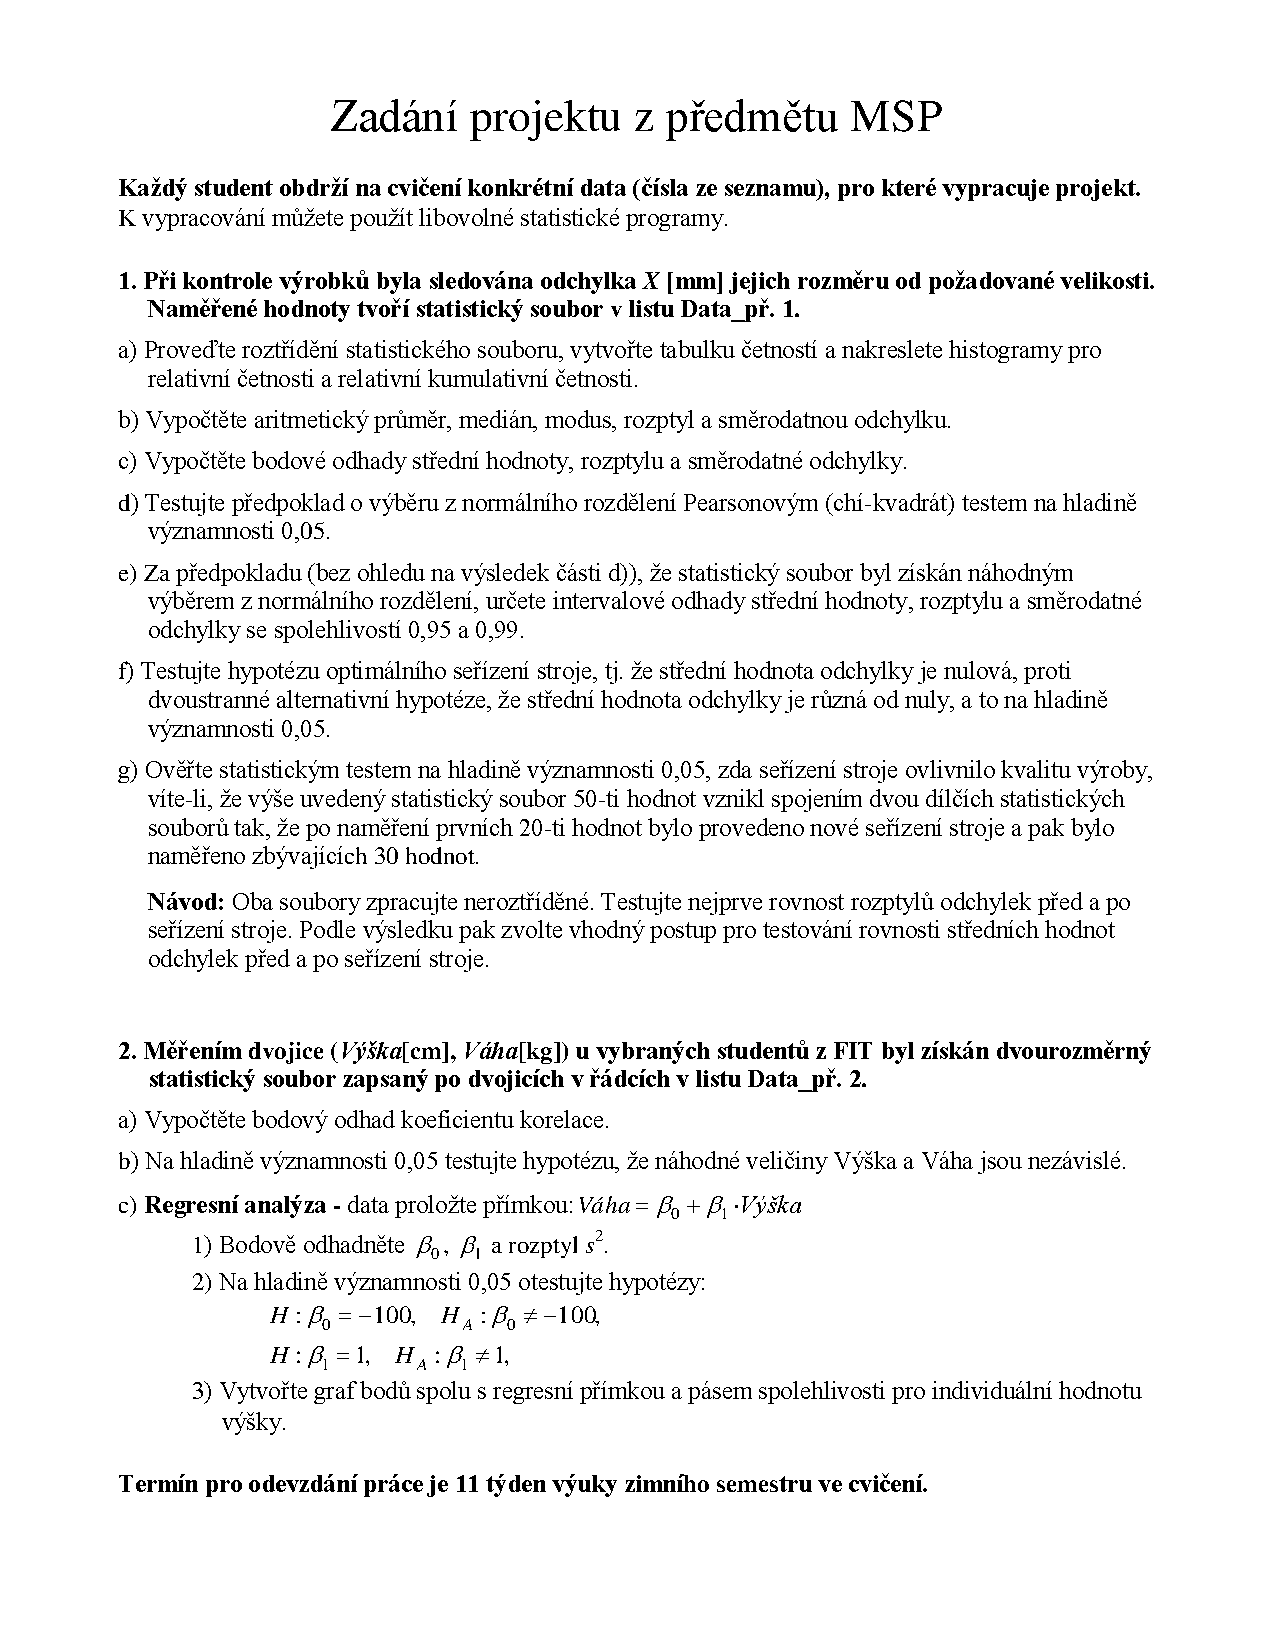
\includepdf[pages=-]{MSP_Projekt_2020-21_Zadani.pdf}

    \section*{Vypracovanie}


    \textbf{1. Při kontrole výrobků byla sledována odchylka $X$ [mm] jejich
    rozměru od požadované velikosti. Naměřené hodnoty tvoří statistický soubor
    v listu Data\_př. 1.}\\

    \begin{table}[H]
        % The minus '-' symbol was causing some issues, this is a fix from
        % https://www.abclinuxu.cz/tex/poradna/show/325037
        \catcode`\-=12
		\begin{tabular}{r|r|r|r|}
			\multicolumn{4}{r}{\thead{\textbf{Štatistický súbor}}} \\[1em]
			\cline{2-2} \cline{4-4}
			1 & $ 0,11 $ & 26 & $ 1,34 $ \\ \cline{2-2} \cline{4-4}
			2 & $ 1,17 $ & 27 & $ 1,94 $ \\ \cline{2-2} \cline{4-4}
			3 & $ 2,57 $ & 28 & $ 1,99 $ \\ \cline{2-2} \cline{4-4}
			4 & $ 1,77 $ & 29 & $ -0,32 $ \\ \cline{2-2} \cline{4-4}
			5 & $ 0,88 $ & 30 & $ 0,7 $ \\ \cline{2-2} \cline{4-4}
			6 & $ 1,45 $ & 31 & $ -0,35 $ \\ \cline{2-2} \cline{4-4}
			7 & $ 1,78 $ & 32 & $ 1,44 $ \\ \cline{2-2} \cline{4-4}
			8 & $ 1,56 $ & 33 & $ 1,63 $ \\ \cline{2-2} \cline{4-4}
			9 & $ 1,01 $ & 34 & $ -0,2 $ \\ \cline{2-2} \cline{4-4}
			10 & $ 2,25 $ & 35 & $ 0,87 $ \\ \cline{2-2} \cline{4-4}
			11 & $ 0,46 $ & 36 & $ -1,34 $ \\ \cline{2-2} \cline{4-4}
			12 & $ 0,23 $ & 37 & $ 2,07 $ \\ \cline{2-2} \cline{4-4}
			13 & $ 0,59 $ & 38 & $ -0,51 $ \\ \cline{2-2} \cline{4-4}
			14 & $ 0,92 $ & 39 & $ 3,31 $ \\ \cline{2-2} \cline{4-4}
			15 & $ 1,84 $ & 40 & $ 0,39 $ \\ \cline{2-2} \cline{4-4}
			16 & $ 2,26 $ & 41 & $ 1,38 $ \\ \cline{2-2} \cline{4-4}
			17 & $ -0,29 $ & 42 & $ -0,98 $ \\ \cline{2-2} \cline{4-4}
			18 & $ 2,06 $ & 43 & $ 0,53 $ \\ \cline{2-2} \cline{4-4}
			19 & $ 0,68 $ & 44 & $ -0,25 $ \\ \cline{2-2} \cline{4-4}
			20 & $ 2,1 $ & 45 & $ 0,59 $ \\ \cline{2-2} \cline{4-4}
			21 & $ 1,88 $ & 46 & $ 1,02 $ \\ \cline{2-2} \cline{4-4}
			22 & $ -0,01 $ & 47 & $ 1,36 $ \\ \cline{2-2} \cline{4-4}
			23 & $ 0,03 $ & 48 & $ 1,38 $ \\ \cline{2-2} \cline{4-4}
			24 & $ 0,36 $ & 49 & $ 1,98 $ \\ \cline{2-2} \cline{4-4}
			25 & $ 0,42 $ & 50 & $ -0,85 $ \\ \cline{2-2} \cline{4-4}
		\end{tabular}
%
		\hspace{4em}
%
        \begin{tabular}{r|r|r|r|}
            \multicolumn{4}{r}{\thead{\textbf{Usporiadaný štatistický súbor}}} \\[1em]
			\cline{2-2} \cline{4-4}
			(1) & $ -1.34 $ & (26) & $ 1.01 $ \\ \cline{2-2} \cline{4-4}
			(2) & $ -0.98 $ & (27) & $ 1.02 $ \\ \cline{2-2} \cline{4-4}
			(3) & $ -0.85 $ & (28) & $ 1.17 $ \\ \cline{2-2} \cline{4-4}
			(4) & $ -0.51 $ & (29) & $ 1.34 $ \\ \cline{2-2} \cline{4-4}
			(5) & $ -0.35 $ & (30) & $ 1.36 $ \\ \cline{2-2} \cline{4-4}
			(6) & $ -0.32 $ & (31) & $ 1.38 $ \\ \cline{2-2} \cline{4-4}
			(7) & $ -0.29 $ & (32) & $ 1.38 $ \\ \cline{2-2} \cline{4-4}
			(8) & $ -0.25 $ & (33) & $ 1.44 $ \\ \cline{2-2} \cline{4-4}
			(9) & $ -0.2 $ & (34) & $ 1.45 $ \\ \cline{2-2} \cline{4-4}
			(10) & $ -0.01 $ & (35) & $ 1.56 $ \\ \cline{2-2} \cline{4-4}
			(11) & $ 0.03 $ & (36) & $ 1.63 $ \\ \cline{2-2} \cline{4-4}
			(12) & $ 0.11 $ & (37) & $ 1.77 $ \\ \cline{2-2} \cline{4-4}
			(13) & $ 0.23 $ & (38) & $ 1.78 $ \\ \cline{2-2} \cline{4-4}
			(14) & $ 0.36 $ & (39) & $ 1.84 $ \\ \cline{2-2} \cline{4-4}
			(15) & $ 0.39 $ & (40) & $ 1.88 $ \\ \cline{2-2} \cline{4-4}
			(16) & $ 0.42 $ & (41) & $ 1.94 $ \\ \cline{2-2} \cline{4-4}
			(17) & $ 0.46 $ & (42) & $ 1.98 $ \\ \cline{2-2} \cline{4-4}
			(18) & $ 0.53 $ & (43) & $ 1.99 $ \\ \cline{2-2} \cline{4-4}
			(19) & $ 0.59 $ & (44) & $ 2.06 $ \\ \cline{2-2} \cline{4-4}
			(20) & $ 0.59 $ & (45) & $ 2.07 $ \\ \cline{2-2} \cline{4-4}
			(21) & $ 0.68 $ & (46) & $ 2.1 $ \\ \cline{2-2} \cline{4-4}
			(22) & $ 0.7 $ & (47) & $ 2.25 $ \\ \cline{2-2} \cline{4-4}
			(23) & $ 0.87 $ & (48) & $ 2.26 $ \\ \cline{2-2} \cline{4-4}
			(24) & $ 0.88 $ & (49) & $ 2.57 $ \\ \cline{2-2} \cline{4-4}
            (25) & $ 0.92 $ & (50) & $ 3.31 $ \\ \cline{2-2} \cline{4-4}
        \end{tabular}
    \end{table}

    \noindent\rule{\linewidth}{0.4pt}\\

    \noindent
    a) Proveďte roztřídění statistického souboru, vytvořte tabulku
    četností a nakreslete histogramy pro relativní četnosti a relativní
    kumulativní četnosti.\\
    
    \noindent
    $ x_{(1)} = \underset{i}{\text{min }}x_i = -1,34 $ \\
    $ x_{(n)} = \underset{i}{\text{max }}x_i = 3,31 $ \\
    Variačný obor: $ \langle{} x_{(1)}, x_{(n)} \rangle{} = \langle{} -1,34;3,31 \rangle{}$ \\
    Rozpätie: $ x_{(n)} - x_{(1)} = 4,65 $ \\
    Počet tried: $ m = 11 $ \\
    Dĺžka triedy: $ \dfrac{x_{(n)} - x_{(1)}}{m} = 0,4227272727 $ \\

    \begin{tabular}[]{|c|c|c|c|c|c|c|c|}
        \hline
        \textbf{trieda} & \textbf{x$_{i-}$} & \textbf{x$_{i+}$} & \textbf{stred triedy} & \textbf{kumul. poč.} & \textbf{poč.} & \textbf{relat. poč.} & \textbf{relat. kumul. poč.} \\
        \hline
        1   &   $-1,3400$ & $-0,9173$   &   $-1,1286$ & $2$ &   $2$ & $0,04$ &  $0,04$ \\
        2   &   $-0,9173$ & $-0,4945$   &   $-0,7059$ & $4$ &   $2$ & $0,04$ &  $0,08$ \\
        3   &   $-0,4945$ & $-0,0718$   &   $-0,2832$ & $9$ &   $5$ & $0,1$ &   $0,18$ \\
        4   &   $-0,0718$ & $0,3509$    &   $0,1395$ &  $13$ &  $4$ & $0,08$ &  $0,26$ \\
        5   &   $0,3509$  & $0,7736$   &    $0,5623$ &   $22$ &  $9$ & $0,18$ &  $0,44$ \\
        6   &   $0,7736$  & $1,1964$   &    $0,9850$ &   $28$ &  $6$ & $0,12$ &  $0,56$ \\
        7   &   $1,1964$  & $1,6191$   &    $1,4077$ &   $35$ &  $7$ & $0,14$ &  $0,7$ \\
        8   &   $1,6191$  & $2,0418$   &    $1,8305$ &   $43$ &  $8$ & $0,16$ &  $0,86$ \\
        9   &   $2,0418$  & $2,4645$   &    $2,2532$ &   $48$ &  $5$ & $0,1$ &   $0,96$ \\
        10  &   $2,4645$   & $2,8873$   &   $2,6759$ &   $49$ &  $1$ & $0,02$ &  $0,98$ \\
        11  &   $2,8873$   & $3,3100$   &   $3,0986$ &   $50$ &  $1$ & $0,02$ &  $1$ \\
        \hline
    \end{tabular}

    \begin{center}
        \noindent
        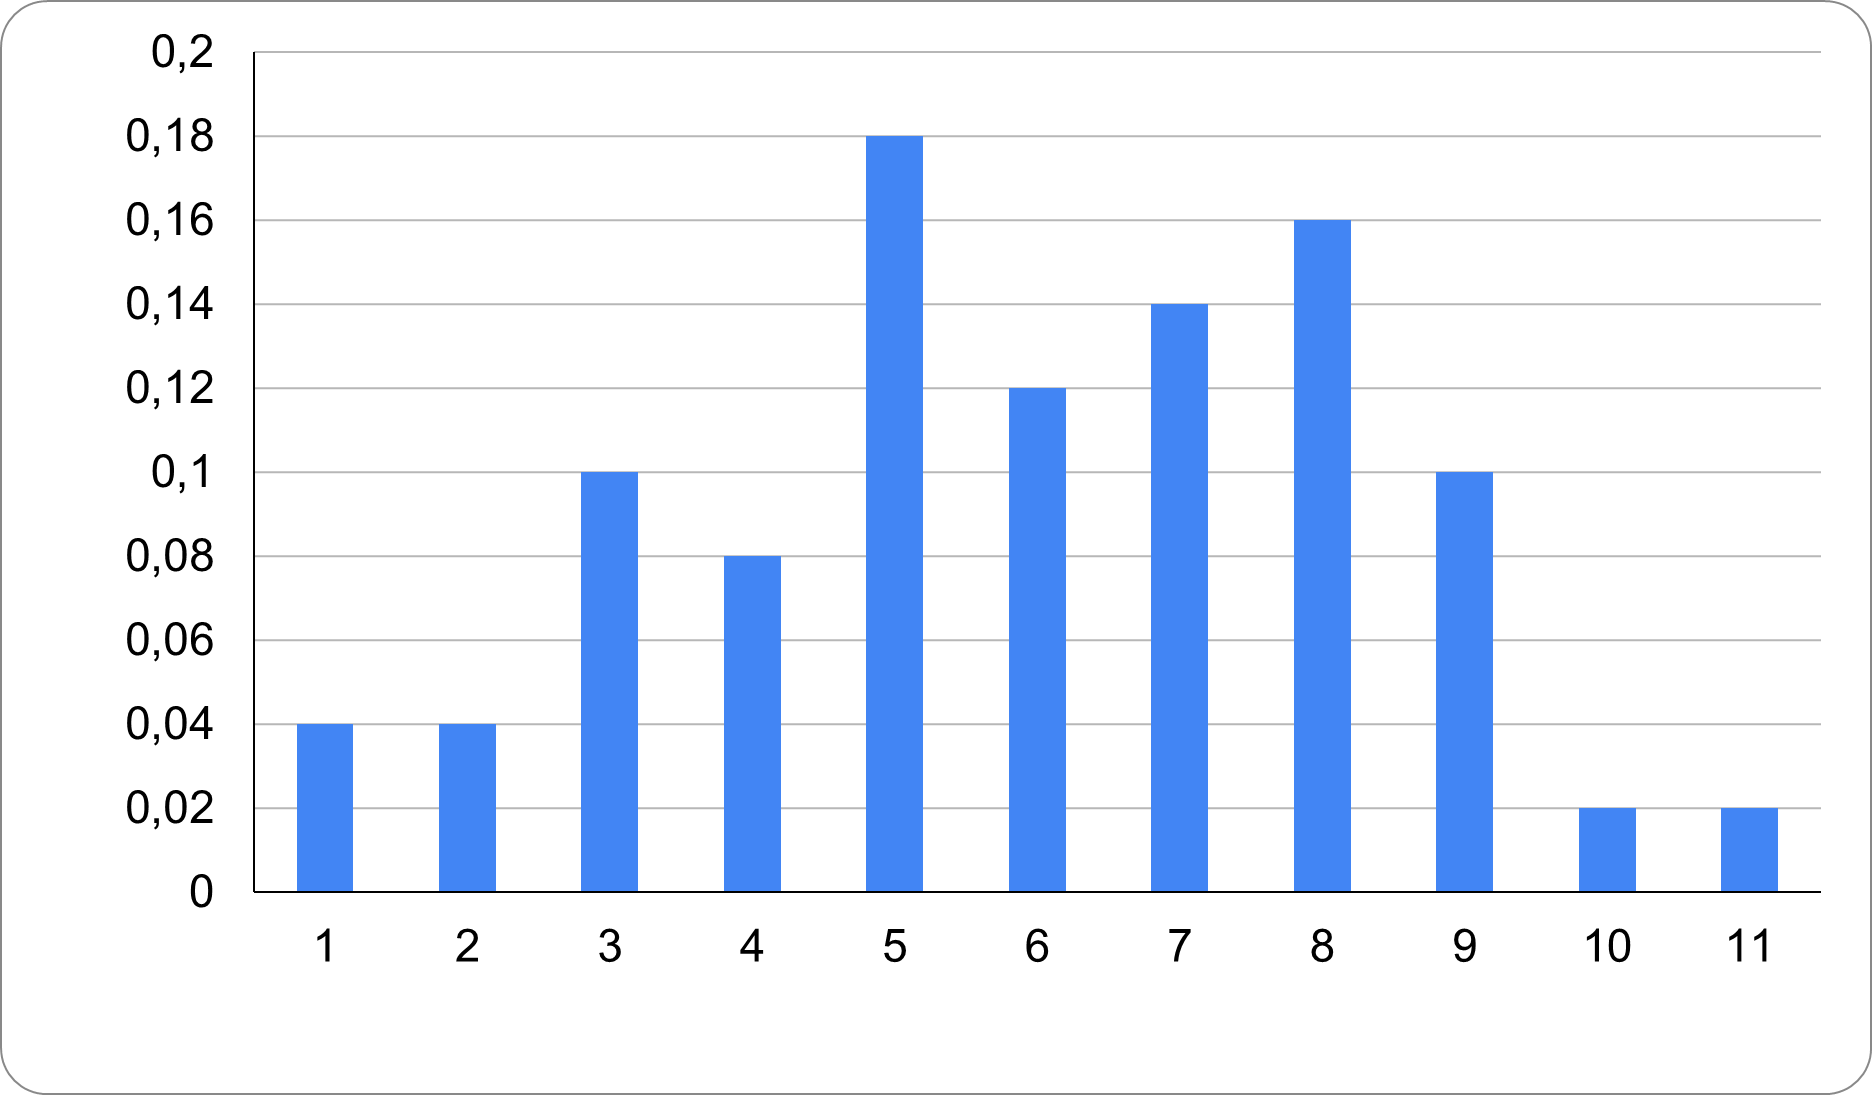
\includegraphics[scale=0.8]{histogram_relat_pocetnost.png}\\\vspace{5pt}
        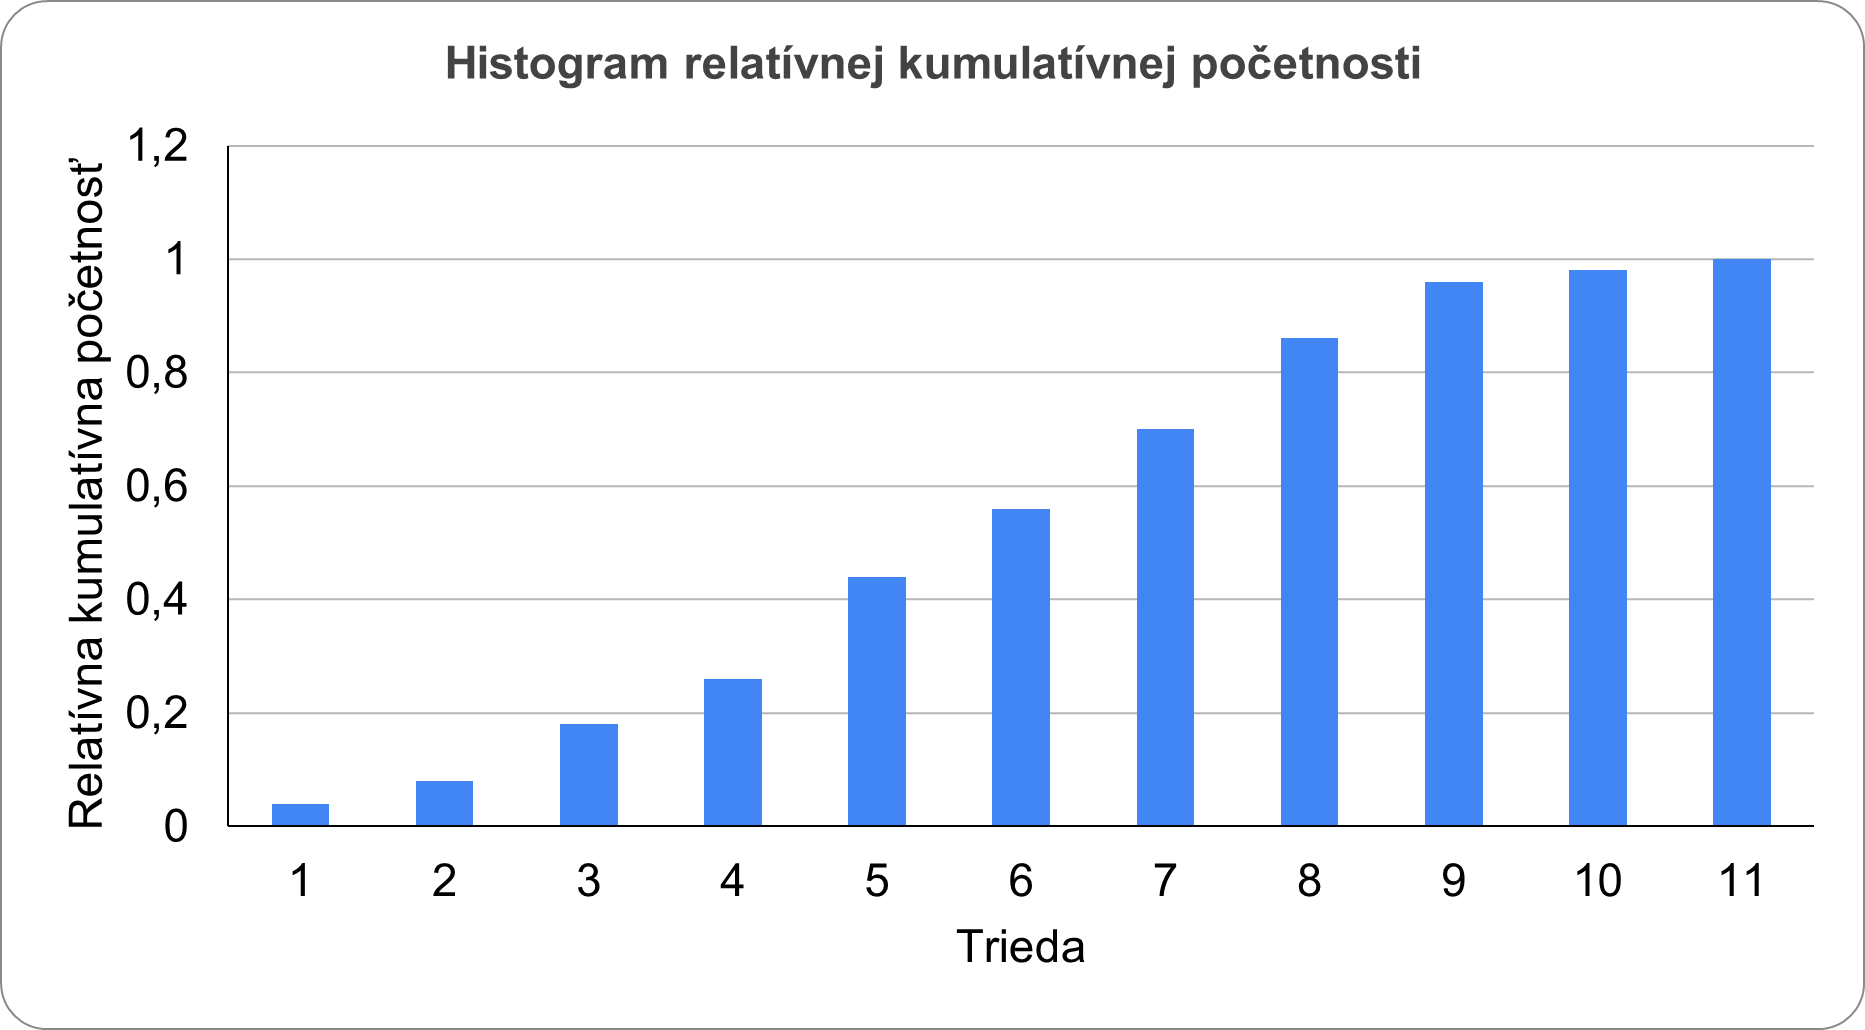
\includegraphics[scale=0.8]{histogram_relat_kumul_pocetnost.png}
    \end{center}

    \noindent\rule{\linewidth}{0.4pt}\\

    \noindent
    b) Vypočtěte aritmetický průměr, medián, modus, rozptyl a směrodatnou
    odchylku.

    \noindent
    $ \overline{x} = \dfrac{1}{n} \sum\limits_{i=1}^{n} x_i = 0,944 $ \\
    Medián: $ \tilde{x} = 0,965 $ \\
    Modus: $ \hat{x} = 0,5623 $ \\
    $ s^2 = \dfrac{1}{n} \sum\limits_{i=1}^{n} (x_i - \overline{x})^2 = 1,0064 $ \\
    $ s = \sqrt{\dfrac{1}{n} \sum\limits_{i=1}^{n} (x_i - \overline{x})^2} = 1,0032 $ \\

    \noindent\rule{\linewidth}{0.4pt}\\

    \noindent
    c) Vypočtěte bodové odhady střední hodnoty, rozptylu a směrodatné odchylky.

    \noindent
    Bodový odhad strednej hodnoty: $ \overline{x} = \dfrac{1}{n} \sum\limits_{i=1}^{n} x_i = 0,944 $ \\
    \noindent
    Bodový odhad rozptylu: $ s^2 = \dfrac{1}{n-1} \sum\limits_{i=1}^{n} (x_i - \overline{x})^2 = 1,027 $ \\
    \noindent
    Bodový odhad smerodatnej odchýľky: $ s = \sqrt{\dfrac{1}{n-1} \sum\limits_{i=1}^{n} (x_i - \overline{x})^2} = 1,0134 $ \\
    
    \noindent\rule{\linewidth}{0.4pt}\\

    \noindent
    d) Testujte předpoklad o výběru z normálního rozdělení Pearsonovým
    (chí-kvadrát) testem na hladině významnosti 0,05.\\

    \begin{tabular}[]{|c|c|c|c|c|c|c|c|}
        \hline
        \textbf{trieda} & \textbf{x$_{i-}$} & \textbf{x$_{i+}$} & \textbf{stred triedy} & \textbf{kumul. poč.} & \textbf{poč.} & \textbf{teor. poč.} & $\dfrac{\text{\textbf{rozdiel}}^2}{\text{\textbf{teor. poč.}}}$ \\
        \hline
        1   &   $-1000$     & $-0,0718$ & $-500,0359$   & $9$   & $9$ & $7,9038$ & $0,1520$ \\
        2   &   $-0,0718$   & $0,3509$  & $0,1395$      & $13$  & $4$ & $6,0556$ & $0,6978$ \\
        3   &   $0,3509$    & $0,7736$  & $0,5623$      & $22$  & $9$ & $7,7029$ & $0,2184$ \\
        4   &   $0,7736$    & $1,1964$  & $0,9850$      & $28$  & $6$ & $8,2542$ & $0,6156$ \\
        5   &   $1,1964$    & $1,6191$  & $1,4077$      & $35$  & $7$ & $7,4509$ & $0,0273$ \\
        6   &   $1,6191$    & $2,0418$  & $1,8305$      & $43$  & $8$ & $5,6658$ & $0,9616$ \\
        7   &   $2,0418$    & $1000$    & $501,0209$    & $50$  & $7$ & $6,9668$ & $0,0002$ \\
        \hline
    \end{tabular}

    \noindent
    Testovacie kritérium: $ t= \sum\limits_{j=1}^{m} \dfrac{(f_j - \hat{f}_j)^2}{\hat{f}_j} = 2,6727$,\\

    \noindent
    $ \chi{}_{1-\alpha}^2 $ pre $ k = 7-2-1 $ stupňov voľnosti: $ 9,4877 $,\\

    \noindent
    doplnok kritického oboru: $ \overline{W_\alpha} = \langle 0;\chi{}_{1-\alpha}^2 \rangle = \langle 0;9,4877 \rangle $.\\

    \noindent
    Keďže $ t \in \overline{W_\alpha} $, tak sa hypotéza $ X \sim N(0,944; 1,027) $ \textbf{nezamieta}.

    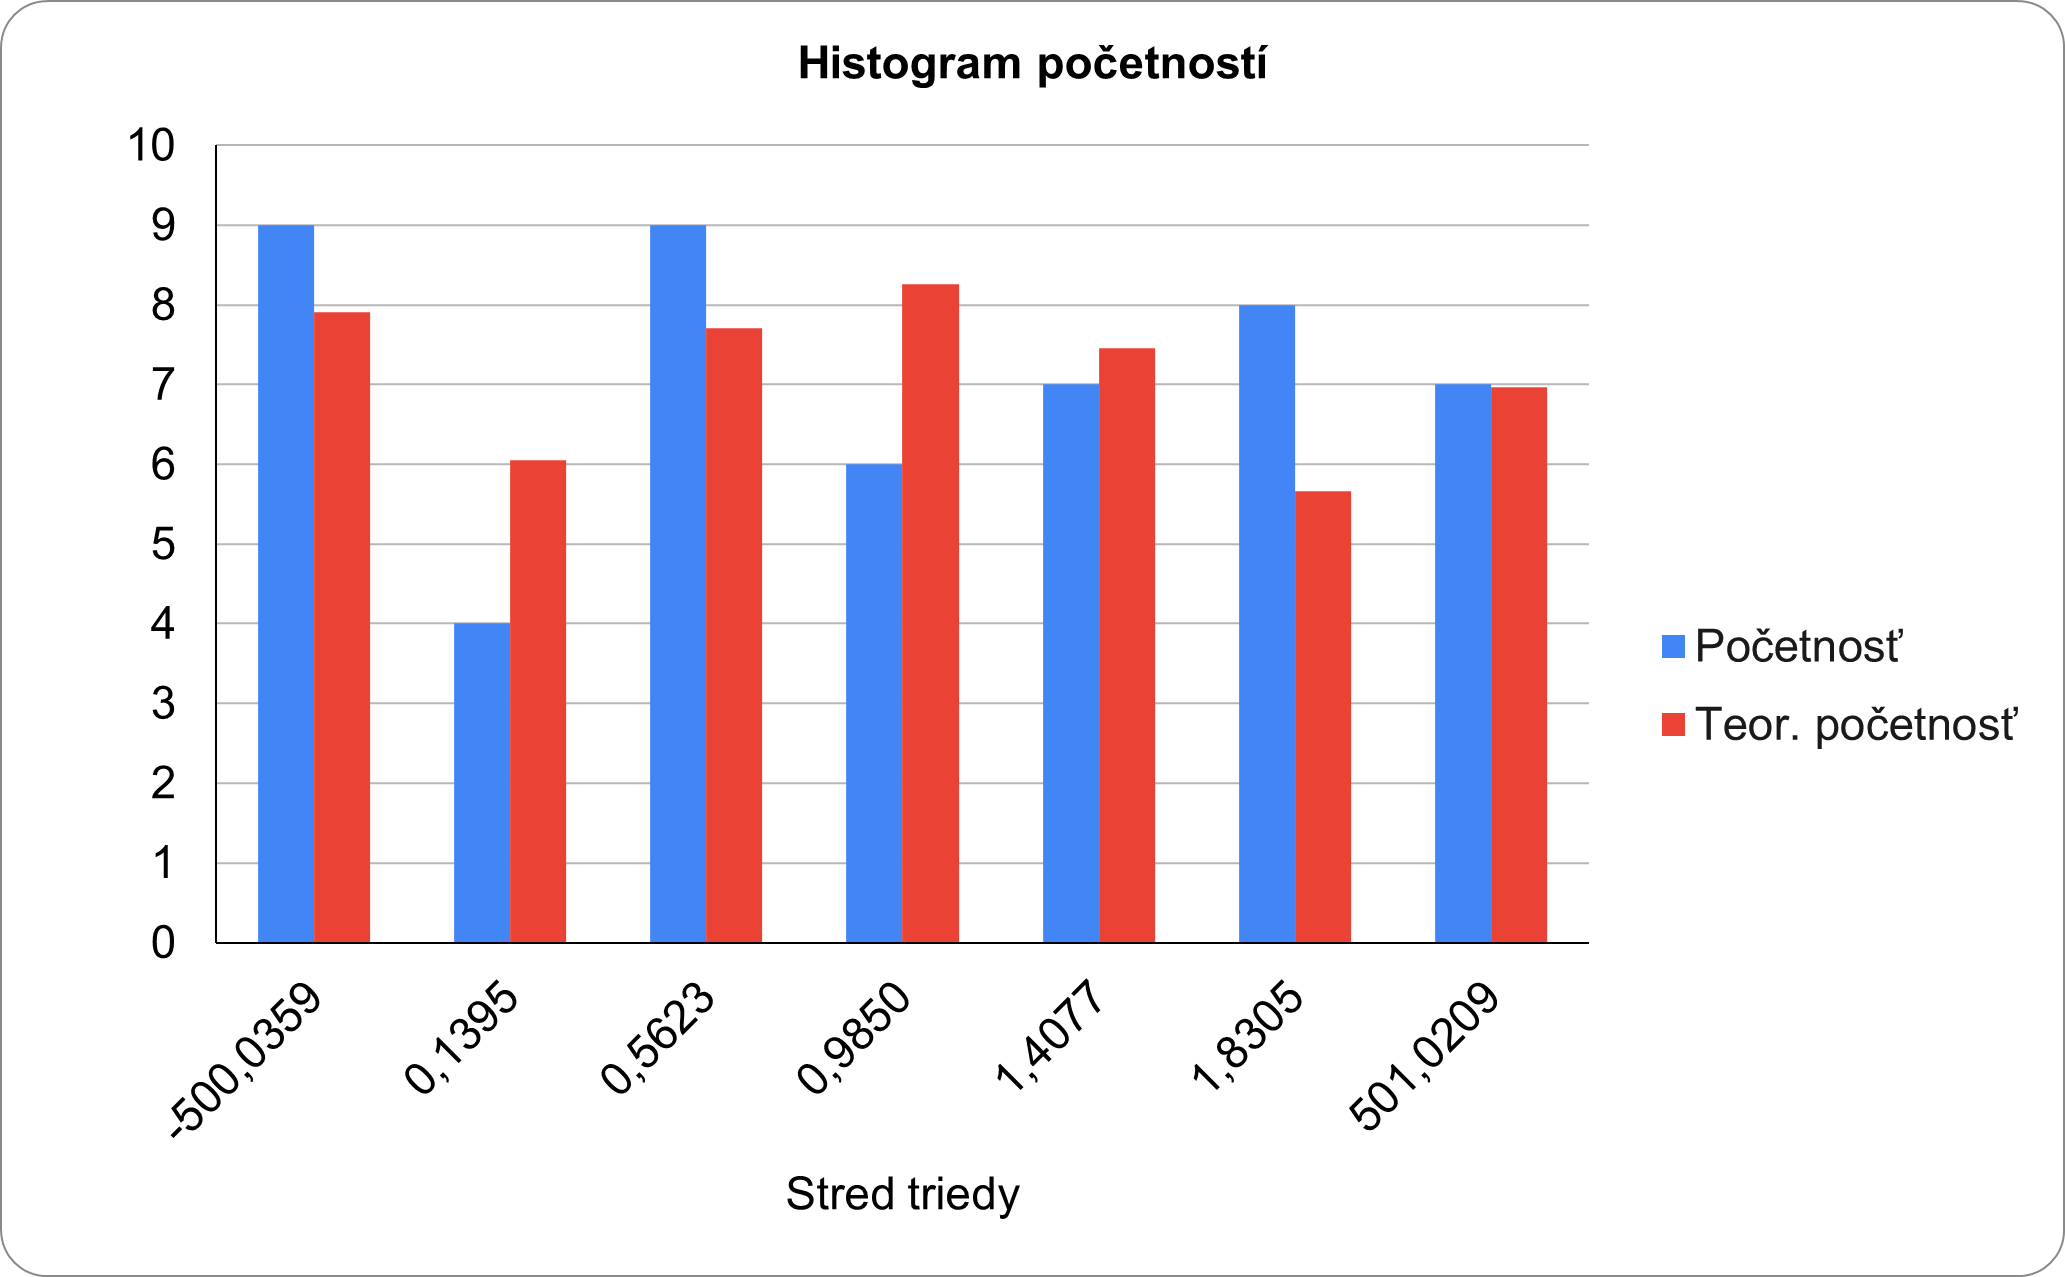
\includegraphics[scale=0.8]{histogram_pocetnosti.png}

    \noindent\rule{\linewidth}{0.4pt}\\

\end{document}
